\chapter{Motivation}

While relationships between emotions and facial expressions or voice changes have been widely explored, 
leading to the availability of feasible methods for real-time automatic analysis, 
full-body movement has not been equally investigated. 
Various studies have shown great potential for inferring about emotions and many other human activities. 
Being able to automatically analyse the origin of movement could improve human performances, 
prevent injuries, promote physical activity, develop cognitive and motor rehabilitation strategies \cite{piana:2016}. 

For this reason, the research in human movement has branches in various fields of study such as biomechanics and neuroscience \cite{vaessen:2019}, 
experimental psychology, and theories from the arts and humanities \cite{camurri:2016}. 

The progress made in this field still does not allow a complete and robust classification of the origin of movement, in an automated way, 
because this relies mainly on arbitrary thresholds to distinguish between different origins and current state of the body, 
like if it is moving or standing still. 
For example, to recognize the instant when a movement starts it is required to manually tune 
minimum speed values that are difficult to automate and generalize for every context. 

Furthermore in movement recognition there are a lot of mid-level features, like the joint angles,
or the limb trajectories or the body segment coordination, which can be extracted and exploited by a comprehensive algorithm 
that weights every feature in an optimize manner, resulting in improved accuracy over all the possible approaches 
that work on them individually, because it could take into account the possible interactions and dependencies between them. 
An holistic approach in this way could leverage the complementary informations present in each feature by weighting them 
based on their relative importance. 
One last point to take into consideration is that algorithms based on single features could end up in overfitting the data
while the comprehensive one has more generalization capability. 

This research aims to contribute to the design of accurate and robust systems for the automated analysis of the origin of movement
by exploiting both the current techniques of analysis and the emerging ML approaches, 
which have become feasible thanks to advancements in computational capabilities of modern machines. 

\section{Roadmap}
From the starting point of our work \cite{kolykhalova:2020}, we re-implemented, improved and modified it to compare the method for identifying the origin of movement obtained based on graphs with our new machine learning-based approach.
The roadmap of this thesis can be outlined as follows: \\
The dataset was initially acquired through manual annotation of movement origins in numerous MoCap videos. 
The results were validated by achieving consensus among multiple annotators. 
Additionally, markers for videos lacking previous labeling were manually assigned and subsequently compressed into clusters.
The central objectives of this thesis encompass the development of:
\begin{itemize}
    \item \textbf{Cluster Stabilization Algorithm} which ensure that clusters, which represent groups of related markers or joints, maintain their consistency and coherence over time. 
    This stability is crucial for accurately tracking and analyzing movements, as it helps prevent spurious or erratic changes in the clusters' characteristics.
    \item \textbf{Graph-based Procedure} to recognize the Origin of Movement by identifying key nodes that play pivotal roles in the motion analysis using an algorithmic method.
    \item \textbf{Machine Learning Approach} to identify the most promising edge of a the skeletal model by finding patterns in data without an algorithmic approach.
\end{itemize}
Given the multifaceted objectives, two parallel pipelines were developed.\\
The first pipeline included the following steps:
\begin{itemize}
    \item Smoothing the time series of each movement using two classical smoothing algorithms.
    \item Extracting physical measurements from the smoothed data.
    \item Applying cosine similarity to pairs of joints linked by arcs based on a model of physical joints in the human body.
    \item Clustering joints for each frame of the movement.
    \item The primary objective here was the temporal stabilization of cluster color changes.
    \item Formation of a second graph with nodes at cluster borders, connected to other clusters. These nodes are weighted based on their connections and ranked across all frames.
\end{itemize}
The second pipeline involved:
\begin{itemize}
    \item Normalizing the dataset in terms of segment length (Time series Sampling), performer's body structure (Skeleton Barycenter and Joints Distance), and the entire trajectory of the movement.
    \item Extracting a wide range of relevant features from the normalized dataset.
    \item Using these features to train a machine learning model.
    \item Evaluating the model's performance using various metrics.
\end{itemize}
Finally, the results from each pipeline are compared.

\clearpage
\begin{figure}[H]
    \centering
    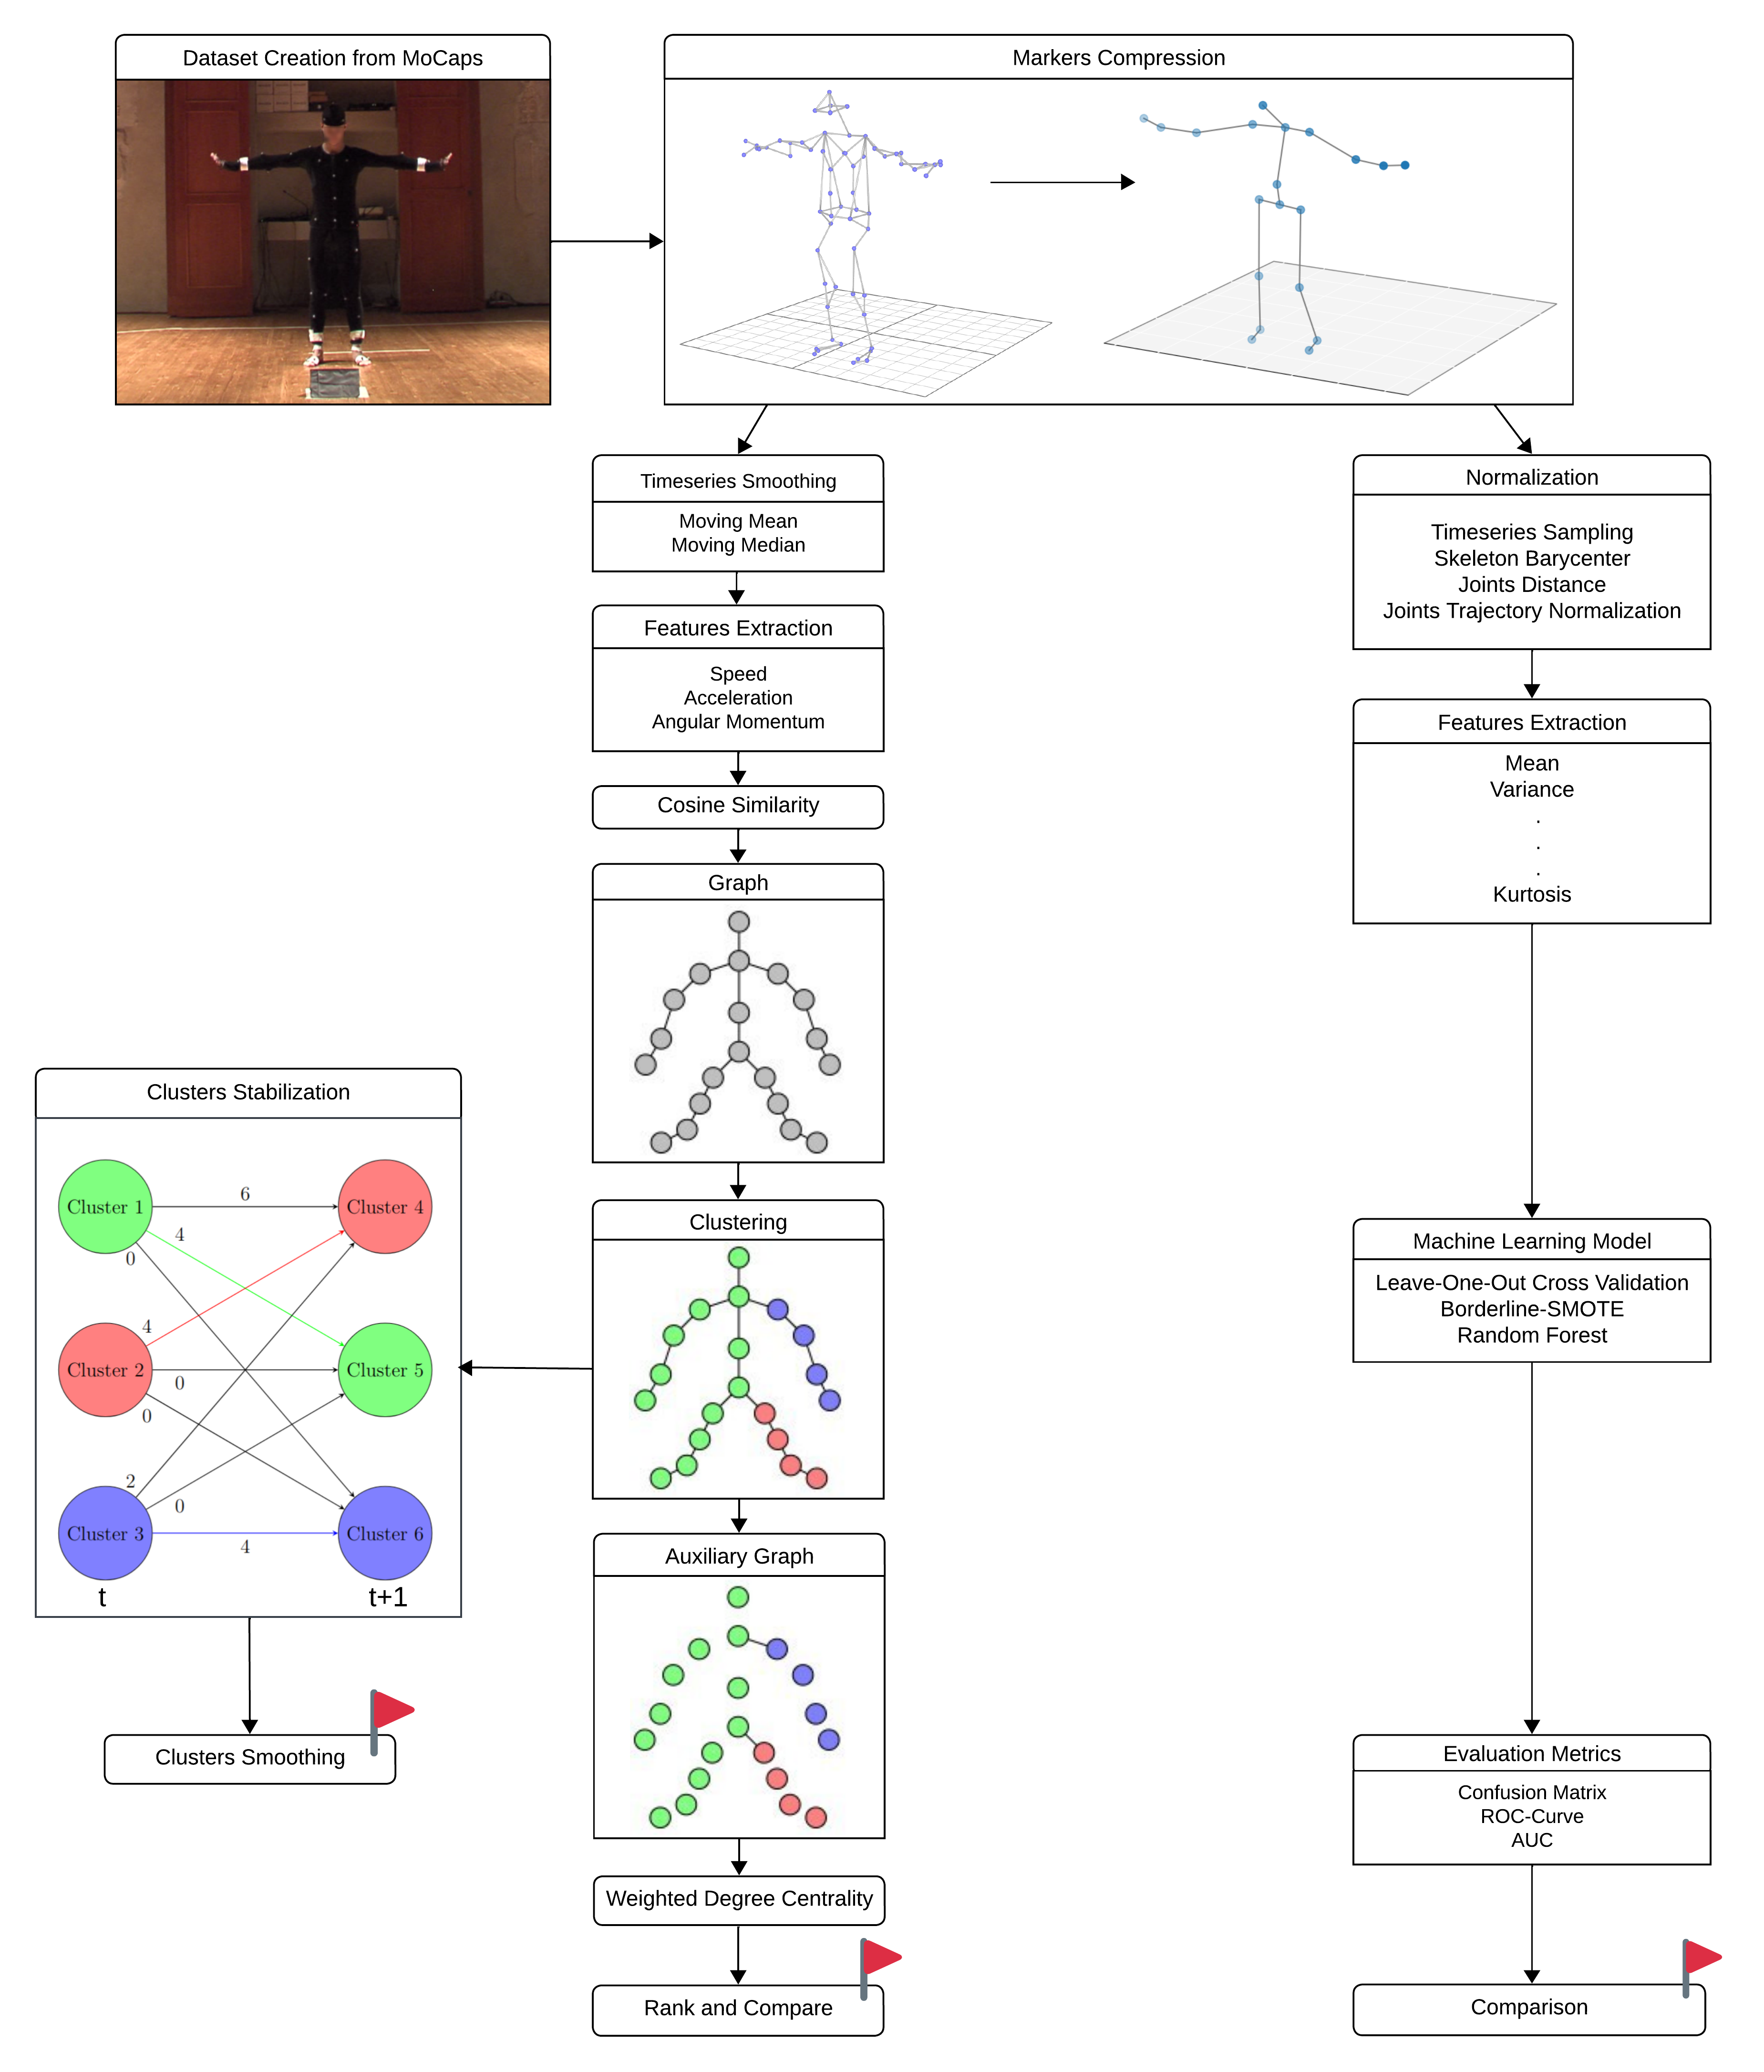
\includegraphics[width=\textwidth,height=\textheight,keepaspectratio]{Walkthrough.png}
    \caption{Roadmap of this Thesis}
    \label{fig:walktrough}
\end{figure}